%-----------------------------------------------------------------------------------------------------
% AUTHOR: Uddalak Mukherjee (uddalakmukherjee49@gmail.com)
%-----------------------------------------------------------------------------------------------------

\documentclass[11pt, oneside]{article}   	% use "amsart" instead of "article" for AMSLaTeX format
\usepackage{geometry}                		% See geometry.pdf to learn the layout options. There are lots.
\geometry{letterpaper}                   		% ... or a4paper or a5paper or ... 
%\geometry{landscape}                		% Activate for rotated page geometry
%\usepackage[parfill]{parskip}    		% Activate to begin paragraphs with an empty line rather than an indent
\usepackage{graphicx}				% Use pdf, png, jpg, or eps§ with pdflatex; use eps in DVI mode
								% TeX will automatically convert eps --> pdf in pdflatex		
\usepackage{amssymb}
\usepackage{color}
\usepackage{enumitem}% http://ctan.org/pkg/enumitem
\usepackage{hyperref} 
\usepackage{graphicx}
\usepackage[rightcaption]{sidecap}

%SetFonts

%SetFonts

\title{Implementing Morlet Kernel in Kernel Principal Component Analysis to de-noise images}
\author{Kernel Kings\\
Biswajit Rana\\
Uddalak Mukherjee}
\date{24th February 2024}							% Activate to display a given date or no date

\begin{document}
\maketitle
%\section{}
%\subsection{}

\section*{Abstract}

We introduce the implementation of a newly proposed kernel in Kernel Principal Component Analysis to filter noisy images. The Morlet Wavelet Function finds extensive application in image processing to filter out noise from distorted or corrupt images. Kernel PCA with standard Gaussian RBF kernel does the same for images likely corrupted with Gaussian noise by reducing the dimensionality of the image hence removing the redundant noises and then reconstructing it. Our project aims to validate some mathematical properties of a kernel constructed using the wavelet function and hence implement it as a valid kernel in Kernel PCA to de-noise images. We will also provide a comparative review of our proposed methodology with Linear PCA and Kernel PCA using Gaussian RBF kernel on the same set of noisy images. 


\section{Introduction}
\cite{PMK} formally introduced the Morlet wavelet kernel based on the Morlet wavelet function $ \psi(x) = \cos(5x)\exp(-\frac{x^2}{2})$  as follows:

\vspace{0.3cm}
\begin{center}
    
$k(x, y)=\prod_{k=1}^d \cos \left(\frac{5\left(x_k-y_k\right)}{a}\right) \exp \left(-\frac{\left(x_k-y_k\right)^2}{2 a^2}\right) \quad \text { where } \hspace{0.3cm} x, y \in \mathbb{R}^d$

    
\end{center}

\vspace{0.3cm}

The paper produced a proof to validate their claim that this is indeed a positive definite kernel using a number of integral transformations. However we have taken a different approach that involves the direct use of Mercer Conditions to prove the same. Once the mathematical foundation for the project is established we will deploy the kernel in kernel principal component analysis to de-noise standard image data corrupted with both Gaussian noise and noise generated from our corresponding wavelet distribution given by: 

\vspace{0.2cm}

\begin{center}
$\chi(x) = \cos(5x)\exp(-\frac{x^2}{2}), \hspace{0.4cm} -2.5 \le x \le 2.5$
\end{center}

\cite{MO} proposed a simple way of mutating data with this type of noise which involves drawing a random sample $x^* \mathtt{\sim} \hspace{0.1cm} Uniform[-2.5,2.5]$ and substituting it in $\chi(x)$ to get a new value $\chi(x^*)$ which will be added as noise to our image data.  

\begin{figure}[h]
    \centering
    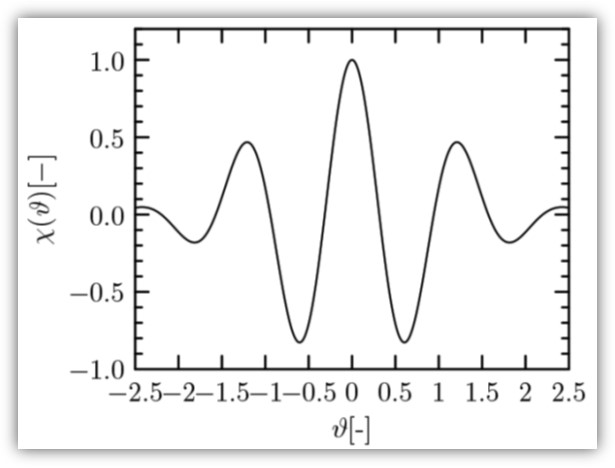
\includegraphics[width=0.3\textwidth]{Morlet.jpg}
    \caption{Morlet Wavelet Density}
    \label{fig:mesh1}
\end{figure}


\section{Proposed methodology}

Once the images are corrupted, they are to be converted to data matrices. The corresponding data matrices then undergo a reduction in dimensionality through Kernel Principal Component Analysis with our suggested kernel. This process removes most of the redundant noises and on reconstruction we are supposed to obtain a nearly noise-free image. Other standard Linear PCA and Kernel PCA models like ones utilizing the Gaussian RBF kernel are also to be tested on the same data and the results are to be compared and interpreted. The dataset to be used for our study is supposed to be a standard de-noising dataset, the choice of which is to be discussed with the instructor. 


\section{Work plan and time line}

Data Collection - 1 week
\\Literature Review - 2 weeks
\\Implementation and Comparison- 2 weeks
\\Interpretation - 1 week


\section{Work plan division in our group}

Data Collection - Uddalak Mukherjee
\\Literature Review - Both
\\Validating Mathematical Foundations - Uddalak Mukherjee
\\Implementation in Python - Biswajit Rana
\\Comparison with other models - Biswajit Rana
\\Interpretation of Results - Both

% \begin{thebibliography}{10}
% \bibitem{PMK}
%  S.Xie, A.T.Lawniczak, S.Krishnan, P.Lio
% \newblock Wavelet Kernel Principal Component Analysis in Noisy Multiscale data Classification
% \newblock{ISRN Computational Mathematics 259 (2012) ID - 197352.}


% \bibitem{MO}
% T.You, Y.HU, P.Li, Y.Tang
% \newblock An improved imperialist competitive algorithm for global optimization
% \newblock{Turkish Journal of Electrical Engineering \& Computer Science (2019) doi:10.3906/elk-1811-59}






\nocite{*}% Biblography without citation!
	
\bibliography{ml_reference} % .bib file
\bibliographystyle{plain}
\end{document}  